%!TEX root = ../main.tex
\chapter{État de l'art}

Comme vous l'aurez compris, deux sujets principaux seront abordés dans ce mémoire : la gestion de la sécurité informatique
dans une chaîne de production DevOps et la gestion opérationnelle de la sécurité de 
cluster Kubernetes. 

Il me semble donc pertinent de dresser un état de l'art pour ces deux sujet afin de permettre une meilleur compréhension des
de leurs problématiques, mais aussi afin à mieux appréhender les possibles solutions à ces dernières.

\section{Les problématiques de sécurité}
\subsection{La sécurisation d'un Pipeline DevOps}

Dans la méthodologie DevOps, le \emph{Pipeline} est un concept regroupant des notions théoriques et socle technique utilisés dans 
le cadre d'un développement logiciel. Ainsi, l'utilisation du terme \emph{Pipeline} fait ainsi reférence au \ac{SDLC}
\autocite[Ch.\ 6]{devops_for_dummies_freeman_forsgren_2019}, aux standards de développement
\autocite[Ch.\ 9]{devops_for_dummies_freeman_forsgren_2019}, processus de qualification et 
validation, de même qu'à l'ensemble des outils et services utilisés par les équipes de développement. Il s'agit donc d'un élément
centrale dans la chaîne de production DevOps: tout problème impactant un élément du \emph{Pipeline} aura des répercutions sur les 
autre et risque ainsi de mettre en péril les opérations de développement.

Nous pouvons donc nous poser la question de la nature de ces risques et particulièrement de ceux relatif à la sécurité du 
\emph{Pipeline}. Pour cela, nous allons utiliser comme support le \ac{SDLC} d'un logiciel afin de mieux cibler les problématiques
de sécurité à chaque étape d'un projet.

\begin{figure}
    \centering
    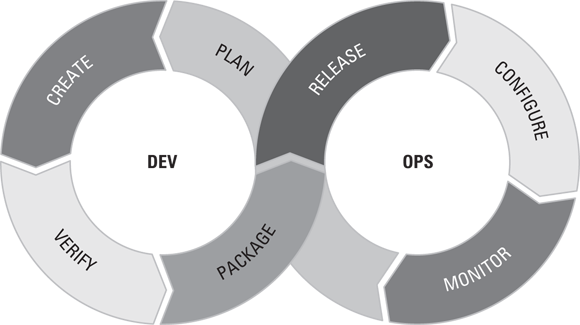
\includegraphics[width=0.5\linewidth]{resources/img/devops_lifecycle.png}
    \caption{Représentation du cycle de vie d'un projet DevOps}
    \label{fig:devops-lifecycle}
  \end{figure}
\newpage

\begin{itemize}
    \begin{minipage}{0.5\linewidth}
        \item item 1
        \item item 2
        \item item 3
    \end{minipage}
    \begin{minipage}{0.5\linewidth}
        \item item 4
        \item item 5
        \item item 6
    \end{minipage}
    \end{itemize}

